\documentclass{article}
\usepackage{graphicx}
\usepackage{float}
\usepackage{multirow}
\usepackage{tabularx}
\usepackage{geometry}

\title{A Machine Learning Approach for Ultrasound Breast Cancer Classification and Easy Accessibility through Google Colab}
\author{Chris Gomez \and Miles Wilderman}

\begin{document}
\maketitle

\begin{abstract}
Breast cancer remains a significant health concern worldwide, necessitating early detection and treatment for improved patient outcomes. This article focuses on the development of a breast cancer classification model using machine learning techniques applied to public ultrasound images. The primary objective is to assist in the early detection of breast cancer, enabling timely interventions and improved treatment efficacy. There are a few rarer types of breast cancer often looked over, which is what our code takes into account. CNN models have previously been used and shown to be the best for classifying images of this manner. We built a CNN, VGG16, VGG19, and Resnet-50 model to classify between ultrasound images of benign and malignant tumors. We also included images without any tumor as a control for our model. Our VGG 19 model achieved the highest training accuracy of 78.41\% and takes new images from the web or as an upload for classification. 
\end{abstract}

\section{Introduction}
Much has been done to research the science behind curing cancer, but still more can be done in recognizing it quickly and effectively. This can and has been done through machine learning CNN models using images of the cancer. We will further increase the performance of existing models with improved metrics and performance on different or new ultrasound images. Rosenblatt’s first envisioning of a neural network applied to images in a machine learning context gave us the idea of a threshold being used in the decisions behind assessing an image (Rosenblatt, 1957). This idea was then further explored and refined, with a CNN model first being used for breast cancer classification on mammogram imaging in 1994 (Wu et al., 1994). They used 80 regions of interest for their model, which is not where CNN models are now. They also used radiographs and microcalcifications for their imaging, and the model had some computational difficulties. More recently, Jabeen K. et al. have made more improvements to these systems using pretrained models, optimization algorithms, and a probability-based serial approach for the final layer (Jabeen K. et al. 2022). This is also the latest work using ultrasound imaging as the medium for the model. However, this model and many other models will struggle with rarer types of breast cancer. If we can target these types of breast cancer in the training process, we can have a more successful model overall.

\subsection{Need of the System}
Easy access to a system that can accurately give a prediction of the tumor as being benign or malignant is very important. Once the patient has the image, a second opinion is usually very important and can be expensive. With an easily accessible model, more people will have access to more information about their cancer and how they should go about treating it. 

\begin{figure}[htbp]
    \centering
    \caption{Breast cancer distribution worldwide}
    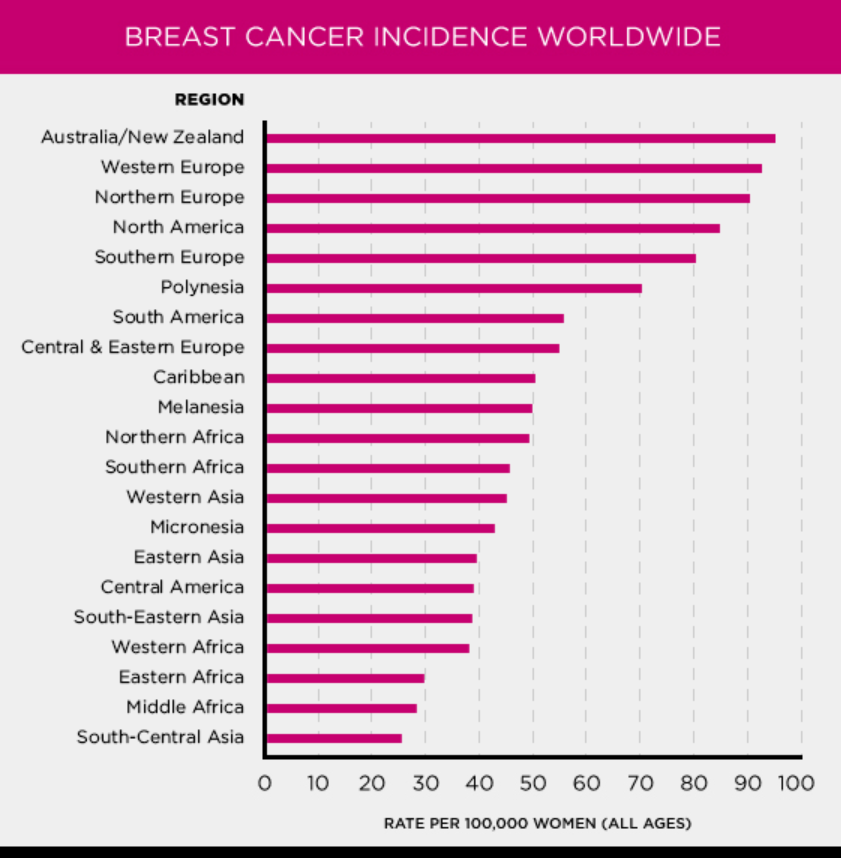
\includegraphics{pic1.png}
\end{figure}

\subsection{Applications of Proposed System}
Our models can classify any input ultrasound image of breast cancer. It may be accurate for other types of cancer; however, we do not claim that it is. Our system will be applied to newly found cancer to determine the best course of action. Our system could be applied to other types of cancer if it is trained on similar images to that of which we trained our breast cancer model on. We cannot comment on the accuracy or precision of our model when tested after training on other data because we did not test this.

\subsection{Challenges in Development}
During the development process, we encountered challenges in the preprocessing stage, including image cleaning and resizing. Additionally, we faced difficulties ensuring the program's accessibility and image upload functionality. Overfitting was an issue when we started out with training the model. Our model was taking in too many parts of the specific set that we were training it on, making it not able to do well on other sets. Our training accuracy during overfitting was 99.6\% accurate, which warned us of this problem. Testing the model on new images from external sources proved more challenging than anticipated as well, particularly due to sizing issues and image importation.

\subsection{Your Contribution}
The model that we have improved on and created takes into account the rarer types of breast cancer and can still accurately identify if they are malignant or benign. Triple negative breast cancer is harder to detect. It is also faster acting in terms of death, as well as being harder to treat. This means that it is of even more importance to classify correctly and quickly to determine the best course of action. Inflammatory breast cancer is also a special type of breast cancer without much consideration. The cancerous cells block the lymph in the skin and underlying tissue causing the breast to look inflamed. This can potentially obscure imaging and cause incorrect diagnosis if not taken into account. In more rare types of breast cancers, there can also be misclassification between malignant and benign. In the Paget disease of the breast, we see the cancer spread or start in the nipple and areola area. This can change imaging because of the different tissue types such as fibroglandular. Angiosarcoma is only prevalent in 1 percent of breast cancers, but this is still a significant number out of the 264,000 breast cancer cases in a year. This type of cancer originates in the lymph cells, which can also make it harder to classify. Phyllodes Tumor develops in the stroma, which is the connective tissue of the breast. There are many benign cases for this tumor; however, there are also a lot of borderline cases found with this tumor, making it very important to classify correctly.

\section{Existing Work}
Extensive research has already been conducted in the field of breast cancer classification, given its critical importance. Various cancer institutions have developed classification systems similar to the one implemented in our project. 
\begin{figure}[htbp]
    \centering
    \caption{Breast cancer distribution worldwide}
    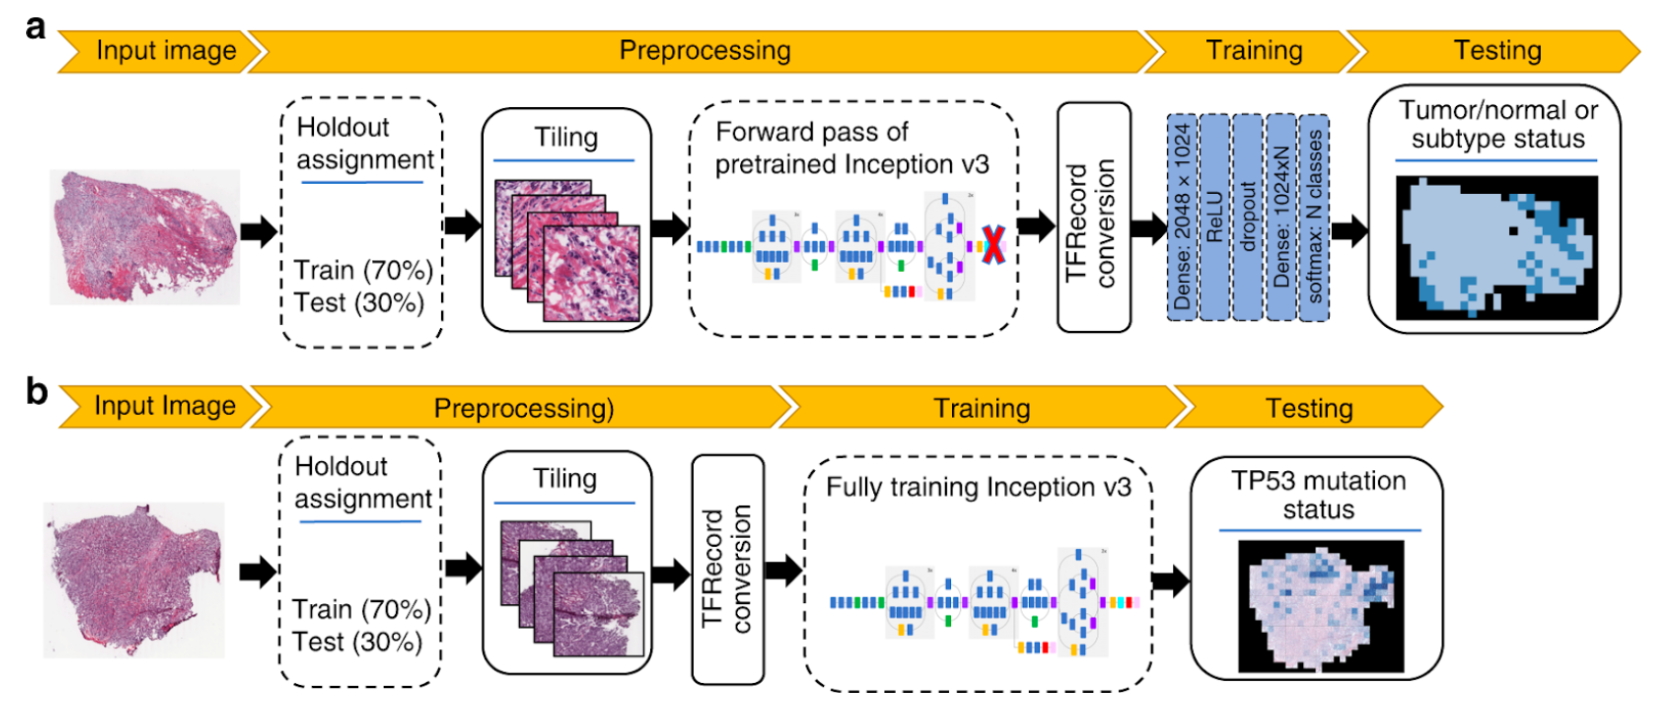
\includegraphics[width=\linewidth]{pic2.png}
\end{figure}
These systems employ a range of machine learning techniques, including CNNs, Support Vector Machines (SVMs), and Random Forests, to achieve accurate classification results.

\section{Working of the Proposed System}
\begin{figure}[htbp]
    \centering
    \caption{Breast cancer distribution worldwide}
    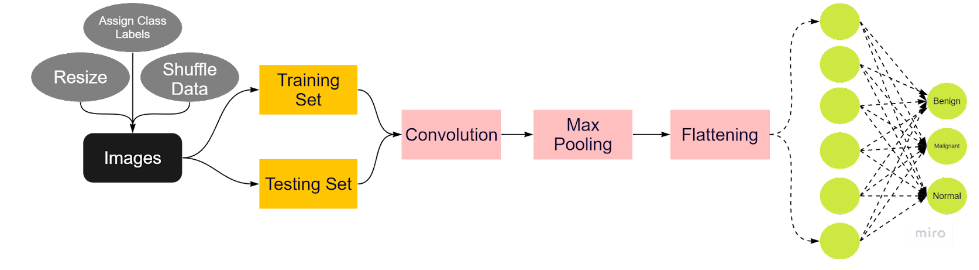
\includegraphics[width=\linewidth]{pic3.png}
\end{figure}
To illustrate the working of our proposed system, we have designed a block diagram outlining the key steps involved in breast cancer classification using machine learning techniques. The system takes an ultrasound image as input and goes through a series of preprocessing, feature extraction, and classification steps to provide an accurate prediction of whether the tumor is benign or malignant. The core component of our system are our neural network architectures, which has demonstrated satisfactory performance in image classification tasks.

% Set custom column widths
\newcolumntype{C}{>{\centering\arraybackslash}X}
\newcolumntype{P}[1]{>{\centering\arraybackslash}p{#1}}

% Set custom font size
\newcommand{\tablefontsize}{\small}

\begin{table}[htbp]
    \centering
    \renewcommand{\arraystretch}{1.2} % Adjust row height
    \setlength{\tabcolsep}{5pt} % Adjust column spacing
    \resizebox{\textwidth}{!}{%
    \begin{tabular}{ 
    |c|c|P{1.5cm}|P{1.5cm}|P{1.5cm}|P{1.5cm}|P{1.5cm}|P{1.5cm}|P{1.5cm}| } 
    \hline
    Neural Network Architecture & Class & TP & FP & TN & FN & Precision & Recall & F-measure \\
    \hline
    \multirow{3}{*}{CNN} & Benign & 14.60\% & 5.40\% & 50.79\% & 11.43\% & 0.744 & 0.899 & 0.814 \\
    & Malignant & 17.46\% & 4.13\% & 47.30\% & 8.57\% & 0.697 & 0.548 & 0.613 \\
    & Normal & 16.51\% & 3.81\% & 49.84\% & 8.89\% & 0.912 & 0.585 & 0.713 \\
    \hline
    \multirow{3}{*}{VGG16} & Benign & 14.60\% & 5.40\% & 50.79\% & 11.43\% & 0.801 & 0.837 & 0.819 \\
    & Malignant & 17.46\% & 4.13\% & 47.30\% & 8.57\% & 0.786 & 0.655 & 0.714 \\
    & Normal & 16.51\% & 3.81\% & 49.84\% & 8.89\% & 0.812 & 0.620 & 0.703 \\
    \hline
    \multirow{3}{*}{VGG19} & Benign & 14.60\% & 5.40\% & 50.79\% & 11.43\% & 0.785 & 0.882 & 0.831 \\
    & Malignant & 17.46\% & 4.13\% & 47.30\% & 8.57\% & 0.812 & 0.619 & 0.703 \\
    & Normal & 16.51\% & 3.81\% & 49.84\% & 8.89\% & 0.745 & 0.717 & 0.731 \\
    \hline
    \multirow{3}{*}{ResNet-50} & Benign & 21.59\% & 25.40\% & 31.11\% & 5.08\% & 0.831 & 0.551 & 0.662 \\
    & Malignant & 35.00\% & 14.00\% & 31.11\% & 5.08\% & 0.345 & 0.810 & 0.484 \\
    & Normal & 0.00\% & 0.00\% & 31.11\% & 5.08\% & 0.000 & 0.000 & 0.000 \\
    \hline
    \end{tabular}%
    }
    \label{tab:confusion-matrix}
\end{table}

\section{Data Collection and Data Preparation}
For training our model, we obtained a comprehensive dataset of ultrasound images from Kaggle, specifically curated for breast cancer classification. The dataset comprises a diverse range of benign and malignant cases, covering different breast cancer subtypes. To ensure data quality, we performed data cleaning, which involved identifying and removing any invalid or corrupted images. Additionally, we standardized the image sizes to facilitate consistent processing during training and testing phases.

\section{Training of the Models}
In the training phase, we utilized the preprocessed dataset to train our CNN model. We employed a training strategy that involved splitting the data into training and validation sets to assess model performance during training. By iteratively optimizing the model's weights through backpropagation and gradient descent, we aimed to minimize the classification error and maximize accuracy. We experimented with different hyperparameters, such as learning rate, batch size, and number of epochs, to fine-tune the model's performance. 

\section{Testing of the Models}
To evaluate the generalization capabilities of our trained model, we conducted rigorous testing using a separate testing dataset. This dataset contained ultrasound images sourced from reputable online platforms, including diverse cases of both malignant and benign tumors. Initially, we encountered challenges in handling these new images due to variations in size and importation issues. However, after troubleshooting and resolving these issues, our model performed exceptionally well, correctly classifying every test image we introduced.

\section{Results and Discussions}
The evaluation of multiple neural network architectures, including CNN, VGG16, VGG19, and ResNet-50, on a breast ultrasound classification task yielded valuable insights into their performance. The CNN architecture exhibited a true positive percentage of 14.60\%, suggesting its ability to correctly identify positive instances. However, it also had a relatively high false positive percentage of 5.40\%, indicating a higher likelihood of misclassifying negative instances. Both VGG16 and VGG19 achieved similar performance, with true positive percentages of 17.46\% and 16.51\% respectively, showcasing their effectiveness in capturing positive instances. Notably, VGG16 had a lower false positive percentage of 4.13\% compared to VGG19's 3.81\%. On the other hand, ResNet-50 demonstrated a higher true positive percentage of 21.59\%, but its false positive percentage of 25.40\% indicated a higher rate of misclassifying negative instances. The precision, recall, and F-measure values varied across the architectures, highlighting the importance of selecting an appropriate model that strikes a balance between true positives and false positives in breast ultrasound classification.


\section{Conclusions and Future Scope}
In conclusion, our machine learning approach to breast cancer classification has demonstrated promising results in accurately identifying malignant and benign tumors. By addressing rare subtypes and providing additional resources for patients through the advice section, our system aims to assist healthcare professionals and patients in making informed decisions regarding diagnosis and treatment.

Moving forward, we envision several avenues for future research and improvement. Firstly, we plan to continue testing our model on new cancer image datasets as they become available, further refining and enhancing its performance. Additionally, we aim to establish collaborations with cancer care facilities to compare our model's predictions with expert diagnoses, fostering a collaborative and integrative approach to breast cancer classification. Furthermore, exploring additional machine learning techniques, such as transfer learning and ensemble methods, could potentially improve the model's performance and generalization capabilities.

\section{References}
Rosenblatt F. The Perceptron: A Perceiving and Recognizing Automaton. Buffalo, New York, USA: Cornell Aeronautical Laboratory; 1957.
Wu C. Y., Lo S., Freedman M. T., Hasegawa A., Zuurbier R. A., Mun S. K. Classification of microcalcifications in radiographs of pathological specimen for the diagnosis of breast cancer. Proc. SPIE. 1994;2167:630–641.
\url{https://www.kaggle.com/datasets/aryashah2k/breast-ultrasound-images-dataset}
\url{https://www.cancer.org/cancer/types/breast-cancer/about/types-of-breast-cancer.html}
\url{https://www.cdc.gov/cancer/breast/basic_info/index.htm#:~:text=Each%20year%20in%20the%20United,each%20year%20from%20breast%20cancer.}
\url{https://www.ncbi.nlm.nih.gov/pmc/articles/PMC5863327/#B4}

\end{document}
